\section{Đề ôn thi giữa kỳ 2 toán 11}
\subsection{Phần trắc nghiệm}
Câu trắc nghiệm nhiều phương án lựa chọn. Học sinh trả lời từ
câu 1 đến câu 12. Mỗi câu hỏi học sinh \textit{chỉ chọn một} phương án.

\Opensolutionfile{ans}[Ans/Dapan]

\hienthiloigiaiex
%%%=============EX_1=============%%%
\begin{ex}%[1H8N1-3]%[Dự án đề kiểm tra toán khối 11 GHKII-NH23-24- Đợt 2-Phạm Tuấn]%[Đề số 5 - Phan Nhật Linh]
	Trong không gian cho ba đường thẳng phân biệt $a, b, c$. Khẳng định nào sau đây đúng?
	\choice
	{Nếu $a$ và $b$ cùng vuông góc với $c$ thì $a \parallel b$}
	{\True Nếu $a \parallel b$ và $c \perp a$ thì $c \perp b$}
	{Nếu góc giữa $a$ và $c$ bằng góc giữa $b$ và $c$ thì $a \parallel b$}
	{Nếu $a$ và $b$ cùng nằm trong $(\alpha)$, $(\alpha) \parallel c$ thì góc giữa $a$ và $c$ bằng góc giữa $b$ và $c$}
	\loigiai{
		Khẳng định đúng là ``Nếu $a \parallel b$ và $c \perp a$ thì $c \perp b$''.
	}
\end{ex}
%%%=============EX_2=============%%%
\begin{ex}%[1D6N3-2]%[Dự án đề kiểm tra toán khối 11 GHKII-NH23-24- Đợt 2-Phạm Tuấn]%[Đề số 5 - Phan Nhật Linh]
	Tập xác định của hàm số $y=(x-1)^{\tfrac{2}{3}}$ là
	\choice
	{$[1;+\infty)$}
	{\True $(1;+\infty)$}
	{$(0;+\infty)$}
	{$\mathbb{R} \setminus\{1\}$}
	\loigiai{
		Điều kiện xác định: $x-1>0 \Leftrightarrow x>1$. \\
		Tập xác định $\mathscr{D}=(1;+\infty)$.
	}
\end{ex}
%%%=============EX_3=============%%%
\begin{ex}%[1D6H1-2]%[Dự án đề kiểm tra toán khối 11 GHKII-NH23-24- Đợt 2-Phạm Tuấn]%[Đề số 5 - Phan Nhật Linh]
	Với $a$ là số thực dương tùy ý, $\sqrt{a^3 \sqrt[4]{a}}$ bằng
	\choice
	{$a^{\frac{13}{6}}$}
	{\True $a^{\frac{13}{8}}$}
	{$a^{\frac{17}{4}}$}
	{$a^{\frac{17}{6}}$}
	\loigiai{
		Ta có $\sqrt{a^3 \sqrt[4]{a}}=\sqrt{a^3 \cdot a^{\frac{1}{4}}}=\sqrt{a^{\frac{13}{4}}}=a^{\frac{13}{8}}$.
	}
\end{ex}
%%%=============EX_4=============%%%
\begin{ex}%[1H8H2-3]%[Dự án đề kiểm tra toán khối 11 GHKII-NH23-24- Đợt 2-Phạm Tuấn]%[Đề số 5 - Phan Nhật Linh]
	Cho hình chóp $S. A B C$ có $S A \perp (A B C)$, tam giác $A B C$ vuông tại $B$. Mệnh đề nào sau đây \textbf{sai}?
	\choice
	{\True $S B \perp A C$}
	{$S A \perp A B$}
	{$S B \perp B C$}
	{$S A \perp B C$}
	\loigiai{
		\immini{
			Vì $S A \perp (A B C)$ nên $S A \perp A B$ và $S A \perp B C$. \\
			Mặt khác $\heva{	&B C \perp A B \\
				&B C \perp S A} \Rightarrow BC \perp (SAB) \Rightarrow B C \perp S B$. \\
			Nếu $SB \perp AC$ thì $\heva{	&AC \perp SB\\
				&AC \perp SA}$\\
			$\Rightarrow AC \perp (SAB) \Rightarrow AC \perp AB$ (Vô lí).
		}
		{
			\begin{tikzpicture}[scale=1,thick,font=\footnotesize, line join=round, line cap=round,>=stealth]
				\path
				(0,3) coordinate (S)
				(0,0) coordinate (A)
				(1.5,-1) coordinate (B)
				(4,0) coordinate (C)
				;
				\draw
				pic[draw=black, angle radius=0.25cm]{right angle=C--B--A};
				\draw (S)--(A)--(B)--(S)--(C)--(B);
				\draw[dashed] (A)--(C);
				\foreach \x/\g in {S/90,A/-120,B/-50,C/0}
				\fill[black] (\x)+(\g:3.5mm) node {$\x$};
			\end{tikzpicture}
		}
	}
\end{ex}
%%%=============EX_5=============%%%
\begin{ex}%[1D6H2-1]%[Dự án đề kiểm tra toán khối 11 GHKII-NH23-24- Đợt 2-Phạm Tuấn]%[Đề số 5 - Phan Nhật Linh]
	Với $a>0$, $\log (100 a)+\log \left(\dfrac{10}{a}\right)$ bằng
	\choice
	{$1000$}
	{$\log \left(100 a+\dfrac{10}{a}\right)$}
	{\True $3$}
	{$1+2 \log a$}
	\loigiai{
		Ta có $\log (100 a)+\log \left(\dfrac{10}{a}\right)=\log \left(100 a \cdot \dfrac{10}{a}\right)=\log 1000=3$.
	}
\end{ex}
%%%=============EX_6=============%%%
\begin{ex}%[1H8H2-2]%[Dự án đề kiểm tra toán khối 11 GHKII-NH23-24- Đợt 2-Phạm Tuấn]%[Đề số 5 - Phan Nhật Linh]
	Cho tứ diện $A B C D$ có $A B=A C$ và $D B=D C$. Khẳng định nào sau đây đúng?
	\choice
	{$A B \perp(A B C)$}
	{$A C \perp B D$}
	{$C D \perp(A B D)$}
	{\True $B C \perp A D$}
	\loigiai{
		\immini{
			Gọi $E$ là trung điểm của $B C$. \\
			Khi đó ta có $\heva{	&A E \perp B C \\
				&D E \perp B C} \Rightarrow B C \perp(A D E) \Rightarrow B C \perp A D$.
		}
		{
			\begin{tikzpicture}[scale=1,thick,font=\footnotesize, line join=round, line cap=round,>=stealth]
				\path
				(0,0) coordinate (A)
				(1.2,-1.5) coordinate (B)
				(4.5,0) coordinate (C)
				($(B)!0.5!(C)$) coordinate (E)
				($(E)+(0,3.5)$) coordinate (D)
				;
				\draw (E)--(D)--(A)--(B)--(D)--(C)--(D)--(C)--(B);
				\draw[dashed] (E)--(A)--(C);
				\foreach \x/\g in {D/90,A/-160,B/-90,C/0,E/-30}
				\fill[black] (\x)+(\g:3.5mm) node {$\x$};
			\end{tikzpicture}
		}
	}
\end{ex}
%%%=============EX_7=============%%%
\begin{ex}%[1D6H4-2]%[Dự án đề kiểm tra toán khối 11 GHKII-NH23-24- Đợt 2-Phạm Tuấn]%[Đề số 5 - Phan Nhật Linh]
	Số nghiệm thực của phương trình $3^{x^2-2}=81$ là
	\choice
	{\True $2$}
	{$1$}
	{$0$}
	{$3$}
	\loigiai{
		Ta có: $$3^{x^2-2}=81 \Leftrightarrow 3^{x^2-2}=3^4 \Leftrightarrow x^2-2=4 \Leftrightarrow x^2=6 \Leftrightarrow x=\pm \sqrt{6}.$$
		Vậy phương trình có 2 nghiệm thực.
	}
\end{ex}
%%%=============EX_8=============%%%
\begin{ex}%[1D6H5-1]%[Dự án đề kiểm tra toán khối 11 GHKII-NH23-24- Đợt 2-Phạm Tuấn]%[Đề số 5 - Phan Nhật Linh]
	Tích tất cả các nghiệm của phương trình $\log ^2 x+2 \log x-3=0$ là
	\choice
	{$-2$}
	{$-3$}
	{\True $\dfrac{1}{100}$}
	{$\dfrac{1}{1000}$}
	\loigiai{
		Điều kiện xác định: $x>0$. \\
		Ta có: $\log ^2 x+2 \log x-3=0 \Leftrightarrow \hoac{	&\log x=1 \\
			&\log x=-3} \Leftrightarrow \hoac{	&x=10 \\
			&x=10^{-3}.}$\\
		Vậy tích hai nghiệm là $\dfrac{1}{1000} \cdot 10=\dfrac{1}{100}$.
	}
\end{ex}
%%%=============EX_9=============%%%
\begin{ex}%[1H8N6-1]%[Dự án đề kiểm tra toán khối 11 GHKII-NH23-24- Đợt 2-Phạm Tuấn]%[Đề số 5 - Phan Nhật Linh]
	Cho hình chóp $S. A B C$ có $S A$ vuông góc với đáy. Góc giữa đường thẳng $S B$ và $(A B C)$ là
	\choice
	{$\widehat{S B C}$}
	{$\widehat{S C A}$}
	{$\widehat{S A B}$}
	{\True $\widehat{S B A}$}
	\loigiai{
		\immini{
			Ta có $S A \perp(A B C)$. \\
			Suy ra góc giữa đường thẳng $S B$ và $(A B C)$ là $\widehat{S B A}$.
		}
		{
			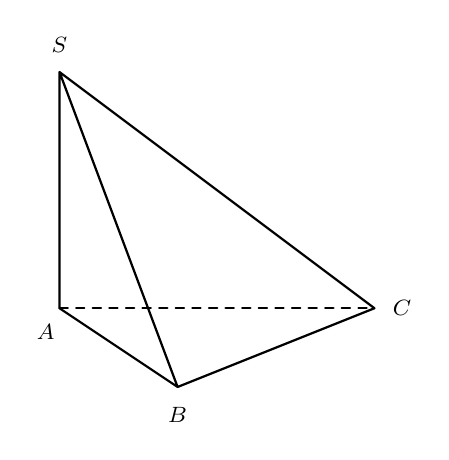
\begin{tikzpicture}[scale=1,thick,font=\footnotesize, line join=round, line cap=round,>=stealth]
				\path
				(0,3) coordinate (S)
				(0,0) coordinate (A)
				(1.5,-1) coordinate (B)
				(4,0) coordinate (C)
				;
				\draw (S)--(A)--(B)--(S)--(C)--(B);
				\draw[dashed] (A)--(C);
				\foreach \x/\g in {S/90,A/-120,B/-90,C/0}
				\fill[black] (\x)+(\g:3.5mm) node {$\x$};
			\end{tikzpicture}
		}
	}
\end{ex}
%%%=============EX_10=============%%%
\begin{ex}%[1D6H4-2]%[Dự án đề kiểm tra toán khối 11 GHKII-NH23-24- Đợt 2-Phạm Tuấn]%[Đề số 5 - Phan Nhật Linh]
	Tập nghiệm của bất phương trình $2^x-5 \leq 0$ là
	\choice
	{\True $S=\left(-\infty; \log _2 5\right]$}
	{$S=\left(0; \log _2 5\right]$}
	{$S=\left[0; \log _2 5\right]$}
	{$S=\left(0; \log _5 2\right]$}
	\loigiai{
		Ta có $2^x-5 \leq 0 \Leftrightarrow 2^x \leq 5 \Leftrightarrow x \leq \log _2 5$. \\
		Tập nghiệm của bất phương trình $2^x-5 \leq 0$ là $S=\left(-\infty; \log _2 5\right]$.
		
	}
\end{ex}
%%%=============EX_11=============%%%
\begin{ex}%[1H8H1-3]%[Dự án đề kiểm tra toán khối 11 GHKII-NH23-24- Đợt 2-Phạm Tuấn]%[Đề số 5 - Phan Nhật Linh]
	Cho hình lập phương $A B C D. A_1 B_1 C_1 D_1$. Góc giữa $A C$ và $D A_1$ là
	\choice
	{$90^{\circ}$}
	{\True $60^{\circ}$}
	{$45^{\circ}$}
	{$120^{\circ}$}
	\loigiai{
		\immini{
			Vì $A_1 C_1 \parallel A C$ nên góc giữa $A C$ và $D A_1$ bằng góc giữa hai đường thẳng $A_1 C_1$ và $D A_1$.\\
			Vì tam giác $D A_1 C_1$ đều nên $\widehat{D A_1 C_1}=60^{\circ}$. \\
			Vậy góc giữa $A C$ và $D A_1$ bằng $60^{\circ}$.
		}
		{
			\begin{tikzpicture}[scale=0.8,thick,font=\footnotesize, line join=round, line cap=round,>=stealth]
				\path
				(0,0) coordinate (O)
				(110: 3cm and 1.5cm) coordinate (A)
				(200: 3cm and 1.5cm) coordinate (B)
				(-70: 3cm and 1.5cm) coordinate (C)
				(20: 3cm and 1.5cm) coordinate (D)
				($(0,3.5)+(110: 3cm and 1.5cm)$) coordinate (A_1)
				($(A_1)+(B)-(A)$) coordinate (B_1)
				($(A_1)+(C)-(A)$) coordinate (C_1)
				($(A_1)+(D)-(A)$) coordinate (D_1)
				;
				\draw (A_1)--(B_1)--(C_1)--(D_1)--(A_1)--(C_1)--(D) (B_1)--(B)--(C)--(C_1) (C)--(D)--(D_1);
				\draw[dashed](A_1)--(A)--(D) (A)--(B) (D)--(A_1) (A)--(C);
				\foreach \x/\g in {A/180,B/190,C/-50,D/0,A_1/100,B_1/160,C_1/-130,D_1/10}
				\fill[black] (\x)+(\g:3.5mm) node {$\x$};
			\end{tikzpicture}
		}
	}
\end{ex}
%%%=============EX_12=============%%%
\begin{ex}%[1H8H1-3]%[Dự án đề kiểm tra toán khối 11 GHKII-NH23-24- Đợt 2-Phạm Tuấn]%[Đề số 5 - Phan Nhật Linh]
	\immini{
		Cho tứ diện $O A B C$ có $O A, O B, O C$ đôi một vuông góc với nhau. Gọi $M, N$ lần lượt là trung điểm của $B C$ và $A C$ (tham khảo hình vẽ bên). Góc giữa hai đường thẳng $O M$ và $A B$ bằng
		\choice
		{$\widehat{A B O}$}
		{$\widehat{M N O}$}
		{$\widehat{N O M}$}
		{\True $\widehat{O M N}$}
	}
	{
		\begin{tikzpicture}[scale=0.8,thick,font=\footnotesize, line join=round, line cap=round,>=stealth]
			\path
			(0,0) coordinate (O)
			(0,3) coordinate (A)
			(1.2,-1.5) coordinate (B)
			(4.5,0) coordinate (C)
			($(B)!0.5!(C)$) coordinate (M)
			($(A)!0.5!(C)$) coordinate (N)
			;
			\draw (A)--(O)--(B)--(A)--(C)--(B);
			\draw[dashed] (O)--(M) (O)--(C);
			\foreach \x/\g in {A/90,B/-90,C/0,O/180,M/-70,N/40}
			\fill[black] (\x) circle(1pt)+(\g:3.5mm) node {$\x$};
		\end{tikzpicture}
	}
	\loigiai{
		\begin{center}
			\begin{tikzpicture}[scale=0.8,thick,font=\footnotesize, line join=round, line cap=round,>=stealth]
				\path
				(0,0) coordinate (O)
				(0,3) coordinate (A)
				(1.2,-1.5) coordinate (B)
				(4.5,0) coordinate (C)
				($(B)!0.5!(C)$) coordinate (M)
				($(A)!0.5!(C)$) coordinate (N)
				;
				\draw (A)--(O)--(B)--(A)--(C)--(B) (M)--(N);
				\draw[dashed] (O)--(M) (O)--(C);
				\foreach \x/\g in {A/90,B/-90,C/0,O/180,M/-70,N/40}
				\fill[black] (\x) circle(1pt)+(\g:3.5mm) node {$\x$};
			\end{tikzpicture}
		\end{center}
		Ta có: $A B \parallel M N$ (do $M N$ là đường trung bình của tam giác $A B C$). \\
		Khi đó $(A B, O M)=(M N, O M)=\widehat{OMN}$.
	}
\end{ex}


\Closesolutionfile{ans}
\bangdapan{Dapan}

\subsection{Câu trắc nghiệm đúng sai}
Học sinh trả lời từ câu 1 đến câu 4.
Trong mỗi ý \circlenum{A}, \circlenum{B}, \circlenum{C} và \circlenum{D} ở mỗi câu, học sinh chọn đúng hoặc sai.
\setcounter{ex}{0}
\LGexTF
\Opensolutionfile{ansbook}[ansbook/DapanDS]
\Opensolutionfile{ans}[Ans/DapanT]
%%%============EX_1==============%%%
\begin{ex}%[1D6V5-1]%[Dự án đề kiểm tra Toán khối 11 GHKII NH23-24-Đợt 2-Nguyễn Tiến]%[Đề số 5-Phan Nhật Linh]
	Cho phương trình $\log^2 _3 x-\log_3 x^2 +2-m=0$. Xét tính đúng sai của các mệnh đề sau
	\choiceTF
	{Khi $m=2$ phương trình có $1$ nghiệm $x=3$}
	{\True Điều kiện xác định của phương trình $x>0$}
	{Với điều kiện xác định của phương trình, đặt $t=\log_2 x$ $(t>0)$, phương trình đã cho có dạng $t^2-2t+2-m=0$}
	{\True Có $2$ giá trị nguyên để phương trình có nghiệm $x\in [1;9]$}
	\loigiai{
		\begin{itemize}
			\item Sai: Thay $m=2$ vào phương trình ta được $\log^2 _3 x-\log_3 x^2=0$.\\
			Điều kiện $x>0$.\\
			Phương trình tương đương với
			$$\log^2 _3 x-2\log_3 x=0 \Leftrightarrow \hoac{& \log_3 x=0\\& \log_3 x=2} \Leftrightarrow \hoac{& x=1\\& x=9.}$$
			\item Đúng: Điều kiện xác định của phương trình là $\heva{& x>0\\& x^2>0} \Leftrightarrow x>0$.
			\item Sai: Với $x>0$, đặt $t=\log_3 x$ phương trình đã cho trở thành $t^2-2t+2-m=0$.
			\item Đúng: Với $x>0$, đặt $t=\log_3 x$.
			\immini{
				Do $x\in [1;9]$ nên $t\in [0;2]$.\\
				Phương trình đã cho trở thành $t^2-2t+2-m=0 \Leftrightarrow t^2-2t+2=m$.\\
				Xét hàm số $f(t)=t^2-2t+2$ có đồ thị như hình bên.\\
				Khi đó để phương trình có nghiệm thì $m\in [1;2]$.\\
				Mà $m\in\mathbb{Z}$ nên $m\in \{1;2\}$.\\
				Vậy có $2$ giá trị nguyên của $m$ thỏa mãn yêu cầu bài toán.
			}{
				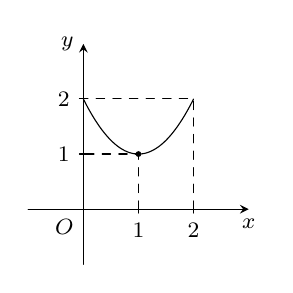
\begin{tikzpicture}[scale=0.7, font=\footnotesize, line join=round, line cap=round, >=stealth]
					\def\a{1} \def\b{-2} \def\c{2} % Hệ số
					\def\xt{-1} \def\xp{3} \def\yt{3} \def\yd{-1} % x_trái, x_phải, y_trên, y_dưới (giới hạn)
					\draw[->] (\xt,0)--(\xp,0) node [below]{$x$};
					\draw[->] (0,\yd)--(0,\yt) node [left]{$y$};
					\node at (0,0) [below left]{$O$};
					\clip (\xt+0.1,\yd+0.1) rectangle (\xp-0.1,\yt-0.1);
					\draw[smooth,samples=300,domain=0:2] plot(\x,{\a*(\x)^2+\b*(\x)+\c});
					\foreach \x in {1,2}
					\draw[shift={(\x,0)},color=black] (0pt,2pt) -- (0pt,-2pt) node [below]{$\x$};
					\foreach \y in {1,2}
					\draw[shift={(0,\y)},color=black] (2pt,0pt) -- (-2pt,0pt) node [left]{$\y$};
					\draw[dashed] (2,0)--(2,2)--(0,2) (1,0)--(1,1)--(0,1);
					\fill (1,1) circle (1.5pt);
				\end{tikzpicture}
			}
		\end{itemize}
	}
\end{ex}
%%%============EX_2==============%%%
\begin{ex}%[1H8H6-1]%[Dự án đề kiểm tra Toán khối 11 GHKII NH23-24-Đợt 2-Nguyễn Tiến]%[Đề số 5-Phan Nhật Linh]
	Cho hình chóp $S.ABC$ có $SA\perp (ABC)$ và $SA=a\sqrt{5}$, đáy là tam giác vuông tại $A$ với $AB=a$, $AC=2a$. Dựng $AK$ vuông góc $BC$ và $AH$ vuông góc $SK$.
	\choiceTF
	{\True Hai đường thẳng $BC$ và $AH$ vuông góc với nhau}
	{\True Đường thẳng $AH$ vuông góc với mặt phẳng $(SBC)$}
	{Đoạn thẳng $AK$ có độ dài bằng $\dfrac{a\sqrt{5}}{5}$}
	{\True Tan góc giữa đường thẳng $SA$ và mặt phẳng $(SBC)$ bằng $\dfrac{2}{5}$}
	\loigiai{
		\immini{
			Ta có $\heva{& BC\perp AK\\& BC\perp SA} \Rightarrow BC\perp (SAK)$.\\
			$\Rightarrow BC\perp AH$, mà $AH\perp SK$.\\
			Nên $AH\perp (SBC)$.\\
			Do đó $SK$ là hình chiếu vuông góc của $SA$ trên $(SBC)$.\\
			Đặt $\alpha=(SA; (SBC))=(SA;SK)=\widehat{ASK}$.\\
			Ta có $AK=\dfrac{AB\cdot AC}{\sqrt{AB^2+AC^2}}=\dfrac{2a\sqrt{5}}{5}$.\\
			Khi đó $\tan\alpha=\dfrac{AK}{AS}=\dfrac{2a\sqrt{5}}{5}\cdot \dfrac{1}{a\sqrt{5}}=\dfrac{2}{5}$.
		}{
			\begin{tikzpicture}[scale=1, font=\footnotesize, line join=round, line cap=round, >=stealth]
				\def\ac{4} % cạnh AC
				\def\ba{2} % cạnh BA
				\def\h{3} % đường cao
				\def\gocA{-45} % góc A của đáy
				\coordinate[label=left:$A$] (A) at (0,0);
				\coordinate[label=below:$B$] (B) at (\gocA:\ba);
				\coordinate[label=right:$C$] (C) at (\ac,0);
				\coordinate[label=above:$S$] (S) at ($(A)+(90:\h)$);
				\coordinate[label=below right:$K$] (K) at ($(B)!1/3!(C)$);
				\coordinate[label=right:$H$] (H) at ($(S)!2/5!(K)$);
				\draw (S)--(A)--(B)--(C)--cycle (K)--(S)--(B);
				\draw[dashed] (A)--(C) (H)--(A)--(K);
				\foreach \diem in {A,B,C,S,H,K}	\fill (\diem)circle(1.2pt);
				\newcommand{\gv}[4][black]{\draw[#1] ($(#3)!8pt!(#2)$)--($(#3)!2!($($(#3)!8pt!(#2)$)!.5!($(#3)!8pt!(#4)$)$)$)--($(#3)!8pt!(#4)$);}
				\gv{S}{A}{K}
				\gv{A}{K}{B}
				\gv{A}{H}{K}
			\end{tikzpicture}
		}
		\noindent
		\begin{itemize}
			\item Đúng: Hai đường thẳng $BC$ và $AH$ vuông góc với nhau.
			\item Đúng: Đường thẳng $AH$ vuông góc với mặt phẳng $(SBC)$.
			\item Sai: Đoạn thẳng $AK$ có độ dài bằng $\dfrac{2a\sqrt{5}}{5}$.
			\item Đúng: Tan góc giữa đường thẳng $SA$ và mặt phẳng $(SBC)$ bằng $\dfrac{2}{5}$.
		\end{itemize}
	}
\end{ex}
%%%============EX_3==============%%%
\begin{ex}%[1D6V3-5]%[Dự án đề kiểm tra Toán khối 11 GHKII NH23-24-Đợt 2-Nguyễn Tiến]%[Đề số 5-Phan Nhật Linh]
	Năm $2024$ bạn Huyền có số tiền $200$ triệu đồng. Do chưa cần sử sụng đến số tiền này nên bạn Huyền gửi tiết kiệm vào một ngân hàng và được nhân viên ngân hàng tư vấn nhiều hình thức gửi khác nhau để bạn Huyền chọn một hình thức gửi.
	\choiceTF
	{\True Nếu bạn Huyền gửi theo kì hạn $6$ tháng với lãi suất không đổi $5\%$ thì số tiền bạn Huyền thu được cả lãi và gốc sau ba năm là $231{,}94$ triệu}
	{\True Sau $48$ tháng bạn Huyền muốn có số tiền là $250$ triệu thì bạn Huyền chọn hình thức lãi kép với lãi suất bằng $1{,}005\%$ một tháng.}
	{Bạn Huyền chọn hình thức gửi theo kì hạn $3$ tháng với lãi suất không đổi là $6\%$ một năm thì sau $13$ quý bạn Huyền có $300$ triệu đồng}
	{Vào ngày $01/01/2024$ bạn Huyền gửi vào ngân hàng với lãi suất không đổi $5\%$ một năm. Hàng tháng vào ngày $01/01$ bạn Huyền rút ra số tiền không đổi là $5$ triệu đồng. Sau $44$ tháng thì bạn Huyền rút hết số tiền đã gửi trong ngân hàng}
	\loigiai{
		\begin{itemize}
			\item Đúng: Ta có $S_6=200\cdot \left(1+5\%\cdot\dfrac{6}{12}\right)^6\approx 231{,}94$.
			\item Đúng: Ta có $250=200\cdot \left(1+r\%\right)^{48} \Leftrightarrow r\approx 1{,}005\%$.
			\item Sai: Ta có $300=200\cdot \left(1+6\%\cdot\dfrac{3}{12}\right)^n \Leftrightarrow n\approx 27{,}2$; tức là gần $9$ quý.
			\item Sai: Ta có $T=200\cdot\left(1+5\%\cdot\dfrac{1}{12}\right)^n-5\cdot\dfrac{\left(1+\dfrac{5\%}{12}\right)^n-1}{\dfrac{5\%}{12}}$.\\
			Khi bạn Huyền rút hết tiền thì $T=200\cdot\left(1+5\%\cdot\dfrac{1}{12}\right)^n-5\cdot\dfrac{\left(1+\dfrac{5\%}{12}\right)^n-1}{\dfrac{5\%}{12}}=0$\\
			$\Rightarrow n\approx 45$ tháng.
		\end{itemize}
	}
\end{ex}
%%%============EX_4==============%%%
\begin{ex}%[1H8V5-5]%[Dự án đề kiểm tra Toán khối 11 GHKII NH23-24-Đợt 2-Nguyễn Tiến]%[Đề số 5-Phan Nhật Linh]
	Cho hình chóp $S.ABCD$ có đáy là hình chữ nhật tâm $I$ biết $AB=a$, $AD=2a$. Gọi $M$ là trung điểm của $AB$ và $N$ là trung điểm của $MI$. Hình chiếu vuông góc của điểm $S$ lên mặt phẳng $(ABCD)$ trùng với điểm $N$. Biết góc tạo bởi đường thẳng $SB$ với mặt phẳng $(ABCD)$ bằng $45^\circ$. Từ $N$ kẻ $NJ\perp AD$, $NH\perp SJ$.
	\choiceTF
	{\True Đường thẳng $AD$ vuông góc với mặt phẳng $(SNJ)$}
	{\True Đường thẳng $NH$ vuông góc với mặt phẳng $(SAD)$}
	{Tam giác $SBN$ là một tam giác vuông cân tại $S$}
	{Khoảng cách giữa hai đường thẳng $MN$ và $SD$ theo $a$ là $\dfrac{a\sqrt{6}}{2}$}
	\loigiai{
		\immini{
			Ta có $MN\parallel AD \Rightarrow MN\parallel (SAD)$.\\
			Nên $\mathrm{d}(MN,SD)=\mathrm{d}(MN,(SAD))=\mathrm{d}(N,(SAD))$.\\
			Ta có $\heva{& AD\perp NJ\\& AD\perp SN} \Rightarrow AD\perp (SNJ)$.\\
			Mà $NH\subset (SNJ)$, suy ra $AD\perp NH$.\\
			Mặt khác $NH\perp SJ$, nên $NH\perp (SAD)$.\\
			Do đó $\mathrm{d}(MN,SD)=\mathrm{d}(N,(SAD))=NH$.\\
			Ta có $SN\perp (ABCD)$ nên hình chiếu của $SB$ lên mặt phẳng $(ABCD)$ là $BN$.\\
			$\Rightarrow \widehat{SBN}=45^\circ$ là góc giữa $SB$ và mặt phẳng đáy.
		}{
			\begin{tikzpicture}[scale=0.9, font=\footnotesize, line join=round, line cap=round, >=stealth]
				\def\bc{5} % cạnh BC
				\def\ba{2.2} % cạnh BA
				\def\h{4} % đường cao
				\def\gocB{45} % góc B của đáy
				\coordinate[label=below:$B$] (B) at (0,0);
				\coordinate[label=left:$A$] (A) at (\gocB:\ba);
				\coordinate[label=below:$C$] (C) at (\bc,0);
				\coordinate[label=right:$D$] (D) at ($(A)+(0:\bc)$);
				\coordinate[label=below:$I$] (I) at ($(A)!0.5!(C)$);
				\coordinate[label=above:$M$] (M) at ($(A)!0.5!(B)$);
				\coordinate[label=above left:$N$] (N) at ($(M)!0.5!(I)$);
				\coordinate[label=above:$S$] (S) at ($(N)+(90:\h)$);
				\coordinate[label=below:$J$] (J) at ($(A)!0.25!(D)$);
				\coordinate[label=right:$H$] (H) at ($(S)!2/3!(J)$);
				\draw (S)--(B)--(C)--(D)--(S)--(C);
				\draw[dashed] (B)--(A)--(D)--(B)--(N) (S)--(A)--(C) (N)--(S)--(J)--(N)--(H) (M)--(I);
				\foreach \diem in {A,B,C,D,S,I,M,N,J,H}	\fill (\diem)circle(1.2pt);
			\end{tikzpicture}
		}
		\noindent
		Xét $\triangle BMN$ vuông ở $M$ có
		$$BN^2=BM^2+MN^2=\left(\dfrac{a}{2}\right)^2+\left(\dfrac{a}{2}\right)^2=\dfrac{a^2}{2} \Rightarrow BN=\dfrac{a}{\sqrt{2}}.$$
		Xét $\triangle SBN$ vuông ở $N$ có $\widehat{SBN}=45^\circ$.\\
		$\Rightarrow \triangle SBN$ vuông cân tại $N$ $\Rightarrow NB=NS=\dfrac{a}{\sqrt{2}}$.\\
		Xét $\triangle SNJ$ vuông ở $N$ có $NJ=AM=\dfrac{AB}{2}=\dfrac{a}{2}$.
		$$\Rightarrow \dfrac{1}{NH^2}=\dfrac{1}{NS^2}+\dfrac{1}{NJ^2}=\dfrac{2}{a^2}+\dfrac{4}{a^2}=\dfrac{6}{a^2} \Rightarrow NH=\dfrac{a\sqrt{6}}{6}.$$
		\begin{itemize}
			\item Đúng: Đường thẳng $AD$ vuông góc với mặt phẳng $(SNJ)$.
			\item Đúng: Đường thẳng $NH$ vuông góc với mặt phẳng $(SAD)$.
			\item Sai: Tam giác $SBN$ là một tam giác vuông cân tại $N$.
			\item Sai: Khoảng cách giữa hai đường thẳng $MN$ và $SD$ theo $a$ là $\dfrac{a\sqrt{6}}{6}$.
		\end{itemize}
	}
\end{ex}

\Closesolutionfile{ans}
\Closesolutionfile{ansbook}

\begin{center}
	\textbf{\textsf{BẢNG ĐÁP ÁN ĐÚNG SAI}}
\end{center}
\input{Ansbook/DapanDS}

%\subsection{Phần tự luận}
%
%\hienthiloigiaibt
%%%=============BT_1=============%%%
\subsection{Câu trả lời ngắn}
\noindent
\textit{Thí sinh trả lời đáp án từ câu 1 đến câu 6}.
\hienthiloigiaibt
%%%==============BT_1==============%%%
\begin{bt}%[1D6V3-2]%[Dự án đề kiểm tra toán khối 11 GHKII-NH23-24- Đợt 2-Nguyễn Trần Anh Tuấn]%[Đề số 5 - Phan Nhật Linh]
	Có bao nhiêu giá trị $m$ nguyên để hàm số $f(x)=\left(2x^2+m x+2\right)^{\tfrac{1}{2}}$ xác định với mọi $x \in \mathbb{R}$?
	\loigiai{
		Do $\dfrac{1}{2} \notin \mathbb{Z}$ nên hàm số đã cho xác định khi $2x^2+m x+2> 0$.\\
		Hàm số đã cho xác định với mọi $x \in \mathbb{R}$ khi $2x^2+m x+2> 0, \forall x \in \mathbb{R}$.\\
		Hay $\Delta=m^2-16 < 0 \Rightarrow -4 < m < 4$.\\
		Mà $m \in \mathbb{Z} \Rightarrow m \in\{-3;-2; \ldots; 2; 3\}$ nên có $7$ giá trị $m$.
	}
\end{bt}
%%%==============BT_2==============%%%
\begin{bt}%[1D6V2-2]%[Dự án đề kiểm tra toán khối 11 GHKII-NH23-24- Đợt 2-Nguyễn Trần Anh Tuấn]%[Đề số 5 - Phan Nhật Linh]
	Biết $x$ và $y$ là hai số thực thỏa mãn $\log _4x=\log _9y=\log _6(x-2y)$. Giá trị của $\dfrac{x}{y}$ bằng
	\loigiai{
		Điều kiện $\heva{&x > 0\\&y > 0\\&x > 2y.}$\\
		Đặt $\log _4x=\log _9y=\log _6(x-2y)=t \Rightarrow \heva{&x=4^t \\&y=9^t \\&x-2y=6^t.}$\\
		Phương trình đã cho trở thành $4^t-2\cdot9^t=6^t \Rightarrow \left(\dfrac{4}{9}\right)^t-\left(\dfrac{2}{3}\right)^t-2=0$.\\
		Giải phương trình trên ta được $\hoac{&\left(\dfrac{2}{3}\right)^t=-1\text { (loại)} \\
			&\left(\dfrac{2}{3}\right)^t=2.}$\\
		Khi đó $\dfrac{x}{y}=\left(\dfrac{4}{9}\right)^t=\left[\left(\dfrac{2}{3}\right)^t\right]^2=4$.
	}
\end{bt}
%%%==============BT_3==============%%%
\begin{bt}%[1D6H3-5]%[Dự án đề kiểm tra toán khối 11 GHKII-NH23-24- Đợt 2-Nguyễn Trần Anh Tuấn]%[Đề số 5 - Phan Nhật Linh]
	 Cho biết tính đến ngày $31$ tháng $12$ năm $2023$, dân số nước ta có khoảng $99\;186\;471$ người và người ta dự đoán tỷ lệ tăng dân số trong vòng $21$ năm, từ năm $2020$ đến năm $2040$ là khoảng $0{,}99 \%$ một năm. Như vậy, nếu tỉ lệ tăng dân số hằng năm không đổi thì đến năm nào dân số nước ta ở mức $ 115 $ triệu người? 
	\loigiai{
		 Chọn năm $2023$ làm mốc tính, tỉ lệ tăng dân số trong vòng $21$, từ năm $2020$ đến năm $2040$ năm là khoảng $0{,}99\%$ một năm, nên dân số nước ta sau $N$ năm $(-3\leq N\leq 17)$ là $S_N=99\;186\;471\cdot (1+0{,}99\%)^N$.\\
		 Để dân số là $115$ triệu người thì $N$ phải thỏa mãn
		\begin{eqnarray*}
			& &115\;000\;000=99\;186\;471\cdot(1+0{,}99\%)^N\\
			& \Rightarrow & \left(1+\dfrac{0{,}99}{100}\right)^N=\dfrac{115\;000\;000}{99\;186\;471}\\
			& \Rightarrow & N \cdot \ln (1{,}0099)=\ln \left(\dfrac{115000000}{99186471}\right) \\
			& \Rightarrow & N=\dfrac{\ln \left(\dfrac{115\;000\;000}{99\;186\;471}\right)}{\ln (1{,}0099)} \approx 15,016 \approx 15.
		\end{eqnarray*}
		Như vậy sau $15$ năm, tức là năm $2038$ thì dân số nước ta ở mức khoảng $115$ triệu người.
	}
\end{bt}
%%%==============BT_4==============%%%
\begin{bt}%[1H4B6-1]%[Dự án đề kiểm tra toán khối 11 GHKII-NH23-24- Đợt 2-Nguyễn Trần Anh Tuấn]%[Đề số 5 - Phan Nhật Linh]
	Cho hình chóp $S.ABC$ có đáy $ABC$ là tam giác đều cạnh bằng $2a$. Tam giác $SAB$ là tam giác vuông cân tại $S$ và nằm trong mặt phẳng vuông góc với đáy. Tính góc giữa đường thẳng $SC$ và mặt phẳng $ABC$?
	\loigiai{
		\begin{center}
			\begin{tikzpicture}[line cap=round,line join=round,scale=.7,>=stealth,font=\footnotesize ]
				\coordinate (A) at (0,0);
				\coordinate (B) at (2.3,-2);
				\coordinate (C) at (5,0);
				\coordinate (H) at ($(A)!0.5!(B)$);%trung điểm
				\coordinate (S) at ($(H)+(0,4.5)$);
				\draw[dashed](H)--(C)--(A);
				\draw (S)--(A)--(B)--(C)--(S)--(B)(S)--(H);
				\foreach \x/\g in {S/90,A/180,H/220,B/-90,C/0}
				\fill[black](\x) circle (1pt)
				($(\x)+(\g:3mm)$) node{\x};
			\end{tikzpicture}
		\end{center}
		Gọi $H$ là trung điểm của $AB$. Do tam giác $SAB$ là tam giác vuông cân tại $S$ và nằm trong mặt phẳng vuông góc với đáy nên ta có $S H=\dfrac{1}{2} AB=a$ và $S H \perp(ABC)$.\\ 
		Suy ra $(SC,(ABC))=SC H$.\\
		$ABC$ là tam giác đều cạnh bằng $2a$ nên $CH=a \sqrt{3}$.\\
		Xét tam giác $SC H$ vuông tại $H$ có $\tan SC H=\dfrac{S H}{C H}=\dfrac{1}{\sqrt{3}}$.\\ Suy ra $(SC,(ABC))=30^{\circ}$.
	}
\end{bt}
%%%==============BT_5==============%%%
\begin{bt}%[1H4K5-5]%[Dự án đề kiểm tra toán khối 11 GHKII-NH23-24- Đợt 2-Nguyễn Trần Anh Tuấn]%[Đề số 5 - Phan Nhật Linh]
	Cho hình chóp $S. ABCD$ có đáy $ABCD$ là hình vuông cạnh $\sqrt{6}$, cạnh bên $SD=2\sqrt{3}$ và $SD$ vuông góc với mặt phẳng đáy. Khoảng cách giữa hai đường thẳng $SB$ và $CD$ bằng
	\loigiai{
		\begin{center}
			\begin{tikzpicture}[scale=1, font=\footnotesize,line join=round, line cap=round, >=stealth]
				\path  (0,0) coordinate (A)
				(0:4) coordinate (B)
				(35:2) coordinate (D)%C
				(D)+(0:4) coordinate (C)
				(D)+(90:3.5) coordinate (S)
				($(S)!(D)!(A)$) coordinate (H)
				;
				\foreach \i in {A,B,C}{\draw[thick] (S)--(\i);}
				\draw[thick] (A)--(B)--(C);
				\draw[dashed,thick] (S)--(D)--(A)	(D)--(C) (D)--(H);
				\pic[draw,thin,angle radius=2mm] {right angle = S--H--D};
				\pic[draw,thin,angle radius=2mm] {right angle = C--D--S};
				\foreach \i/\g in {S/90,D/135,A/-135,B/-45,C/45,H/110}{\draw[fill=black](\i) circle (1pt) ($(\i)+(\g:3mm)$) node[scale=1]{$\i$};}
			\end{tikzpicture}
		\end{center}
		Ta có $\heva{&AB \perp SD \\&A B \perp AD \\&SD \cap AD=D \text { trong }(SAD)} \Rightarrow AB \perp(SAD)$.\\
		Vẽ $DH \perp S A$ tại $H$ trong mặt phẳng $(SAD)$.\\
		Ta có $\heva{&DH \perp AB \\&D H \perp S A \\	&A B \cap S A=A \text { trong }(SAB)} \Rightarrow DH \perp(S AB)$.\\
		Vì $CD \parallel (SAB)$ nên $d(SB; CD)=d((SAB); CD)=d((SAB); D)=DH$.\\
		$\triangle SAD$ vuông tại $D$ với đường cao $DH$ có $DH=\dfrac{SD \cdot DA}{\sqrt{SD^2+DA^2}}=\dfrac{2 \sqrt{3} \cdot \sqrt{6}}{\sqrt{(2 \sqrt{3})^2+(\sqrt{6})^2}}=2$.
	}
\end{bt}
%%%==============BT_6==============%%%
\begin{bt}%[1H8H2-2]%[Dự án đề kiểm tra toán khối 11 GHKII-NH23-24- Đợt 2-Nguyễn Trần Anh Tuấn]%[Đề số 5 - Phan Nhật Linh]
	Ông A muốn xây một cái bể chứa nước lớn dạng một khối hộp chữ nhật không nắp có thể tích bằng $2304$ m$^3$. Đáy bể là hình chữ nhật có chiều dài gấp đôi chiều rộng, giá thuê nhân công để xây bể là $600\;000$ đồng/m$^2$. Nếu ông A biết xác định các kích thước của bể hợp lí thì chi phí thuê nhân công sẽ thấp nhất. Hỏi ông A trả chi phí thấp nhất (đơn vị: triệu đồng) để xây dựng bể đó là bao nhiêu (biết độ dày thành bể và đáy bể không đáng kể)?
	\loigiai{
		Theo bài ra ta có để chi phí thuê nhân công là thấp nhất thì ta phải xây dựng bể sao cho tổng diện tích xung quanh và diện tích đáy là nhỏ nhất.\\
		Gọi ba kích thước của bể là $a$, $2a$ $c$ (đơn vị mét, $a>0$, $c>0$).\\
		Ta có diện tích các mặt cần xây là $S=2a^2+4a c+2a c=2a^2+6a c$.\\
		Thể tích bể $V=a \cdot 2a \cdot c=2a^2c=2304\Rightarrow c=\dfrac{1152}{a^2}$.\\
		Suy ra $S=2a^2+6a \cdot \dfrac{1152}{a^2}=2a^2+\dfrac{6912}{a}=2a^2+\dfrac{3456}{a}+\dfrac{3456}{a} \geq 3\cdot \sqrt[3]{2a^2\cdot \dfrac{3456}{a} \cdot \dfrac{3456}{a}}=864$.
		Vậy $S_{\min}=864$ m$^2$, khi đó chi phí thấp nhất là $864\cdot 600\;000=518{,}4$ triệu đồng.
	}
\end{bt}